\hsection{Our First Program}%
\label{sec:ourFirstProgram}%
\FloatBarrier%
%
We now want to write and execute our very first \python\ program.
This program should just print \inQuotes{Hello World!} to the text output and then exit.
It therefore will consist of the single statement \pythonil{print("Hello World!")}, as illustrated in \cref{lst:very_first_program}.

\gitPythonAndOutput{\programmingWithPythonCodeRepo}{00_veryFirstProject}{very_first_program.py}{--args format}{very_first_program}{%
Our very first \python\ program, which just prints \inQuotes{Hello World!}}%
%
\begin{figure}%
\centering%
%
\subfloat[][%
Creating a new project in \pycharm, step~1: click \menu{New Project}.%
\label{fig:firstProgram01createPycharmProject}%
]{\tightbox{\includegraphics[width=0.47\linewidth]{\currentDir/firstProgram01createPycharmProject}}}%
%
\strut\hfill\strut%
%
\subfloat[][%
Creating a new project in \pycharm, step~2: Make sure that \menu{Pure Python} is selected in the left pane, then select a name for the project (here: \directory{00\_veryFirstProject}), a directory location (some path on my \ubuntu\ machine, you will pick some other directory), and we select the current \python\ installation as \menu{Custom Environment}. %
We finally click \menu{Create}.%
\label{fig:firstProgram02createPycharmProject}%
]{\tightbox{\includegraphics[width=0.47\linewidth]{\currentDir/firstProgram02createPycharmProject}}}%
%
\\[10pt]%
%
\subfloat[][%
The new and empty project has been created.%
\label{fig:firstProgram03pycharmProjectCreated}%
]{\tightbox{\includegraphics[width=0.775\linewidth]{\currentDir/firstProgram03pycharmProjectCreated}}}%
%
\\[10pt]%
%
\subfloat[][%
We create a new \python\ file within this project by right-clicking on the project folder \directory{00\_veryFirstProject} and selecting \menu{New>Python File}.%
\label{fig:firstProgram04createPythonFile}%
]{\tightbox{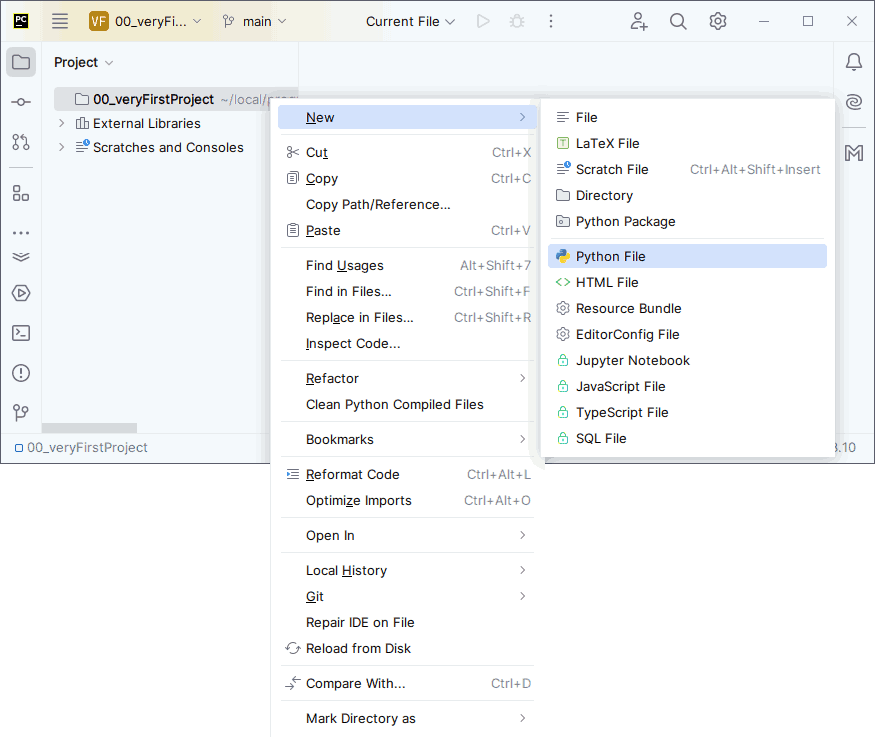
\includegraphics[width=0.775\linewidth,trim={0 200 0 0},clip]{\currentDir/firstProgram04createPythonFile}}}%
%
\caption{The steps to create a new \python\ file in a new \pycharm\ project and to then run it (\ubuntu).}%
\label{fig:veryFirstProgramA}%
\end{figure}
%
\begin{figure}%
\ContinuedFloat%
\centering%
%
\subfloat[][%
We enter a name for the new \python\ file (here:~\directory{very\_first\_program}) and hit \keys{\enter}.%
\label{fig:firstProgram05createPythonFile}%
]{\tightbox{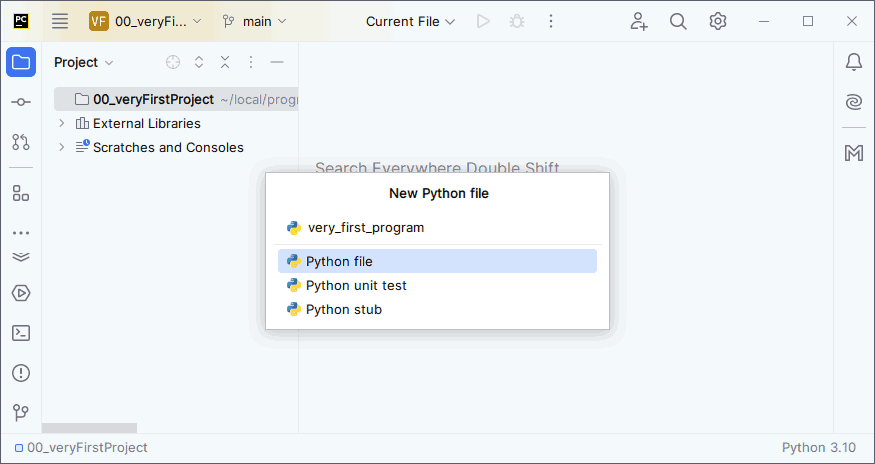
\includegraphics[width=0.775\linewidth]{\currentDir/firstProgram05createPythonFile}}}%
%
\\[10pt]%
%
\subfloat[][%
The new and empty file \directory{very\_first\_program.py} has been created in the project \directory{00\_veryFirstProject}.%
\label{fig:firstProgram06pythonFileCreated}%
]{\tightbox{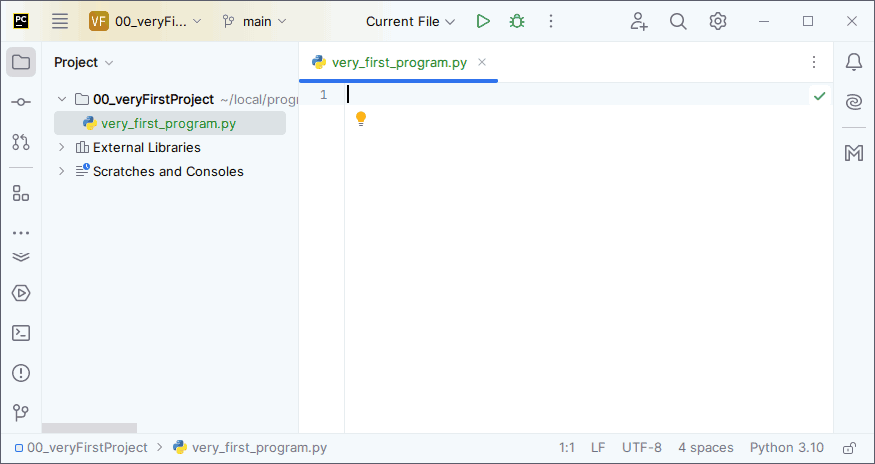
\includegraphics[width=0.775\linewidth]{\currentDir/firstProgram06pythonFileCreated}}}%
%
\\[10pt]%
%
\subfloat[][%
We enter the text from \cref{lst:very_first_program}. \pycharm\ automatically saves it.%
\label{fig:firstProgram07writeHelloWorld}%
]{\tightbox{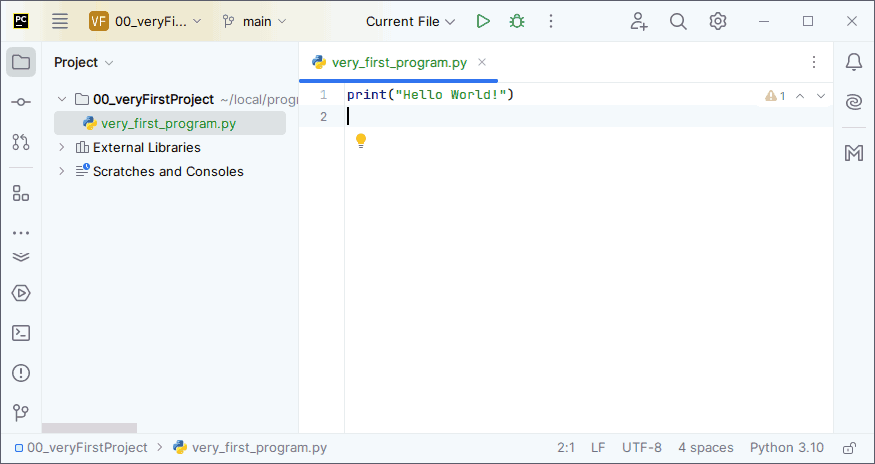
\includegraphics[width=0.775\linewidth]{\currentDir/firstProgram07writeHelloWorld}}}%
%
%
\caption{The steps to create a new \python\ file in a new \pycharm\ project and to then run it (\ubuntu,~continued).}%
\label{fig:veryFirstProgramB}%
\centering%
%
\end{figure}%
%
\begin{figure}%
\ContinuedFloat%
\centering%
%
\subfloat[][%
In order to run this program, we right-click on the program file in the tree view and select \menu{Run `very\_first\_program'}. %
Alternatively, we could press \keys{\ctrl+\shift+F10}.%
\label{fig:firstProgram08runProgram}%
]{\tightbox{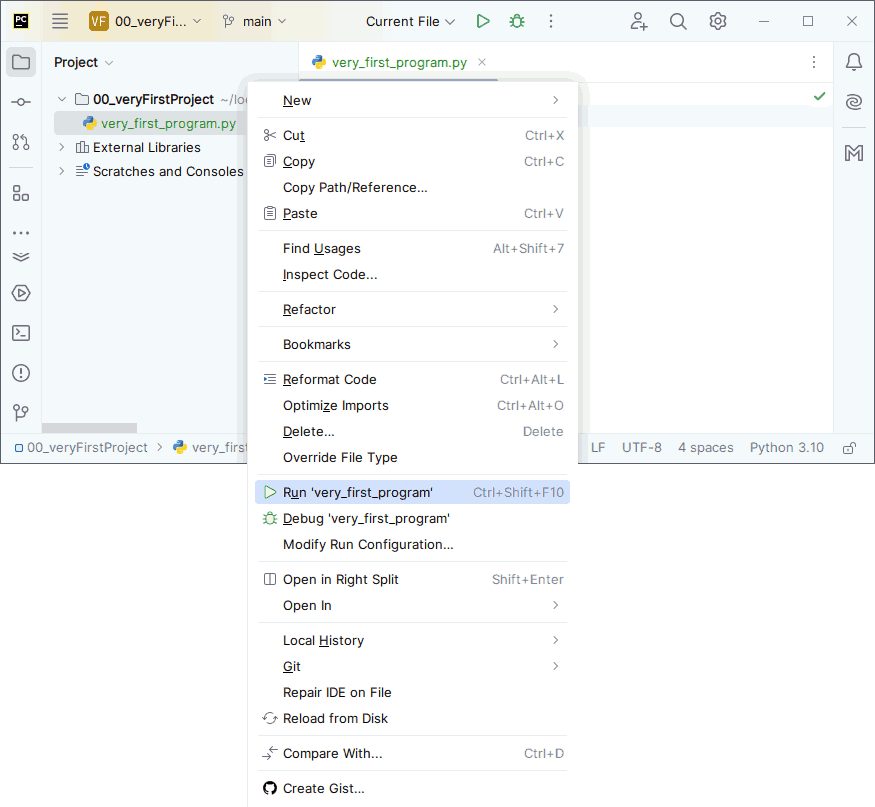
\includegraphics[width=0.775\linewidth,trim={0 200px 0 0},clip]{\currentDir/firstProgram08runProgram}}}%
%
\\[10pt]%
%
\subfloat[][%
And indeed, in the console pane at the bottom of the \pycharm\ window, the text \inQuotes{Hello World!} appears.%
\label{fig:firstProgram09programResult}%
]{\tightbox{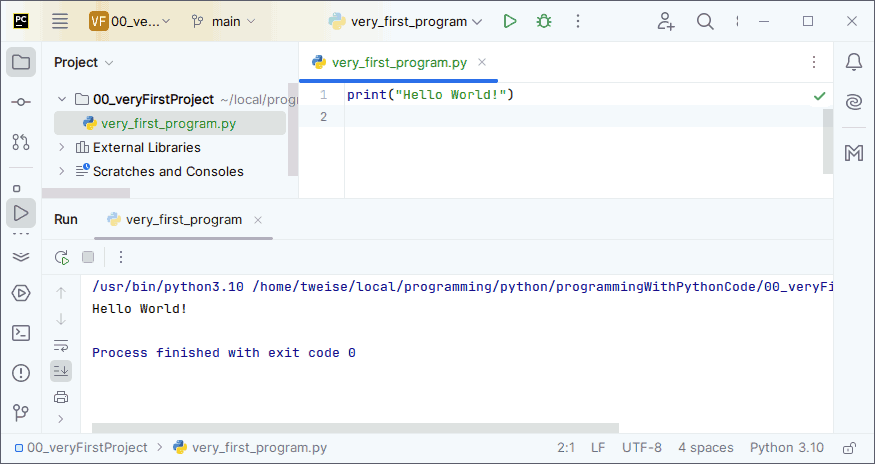
\includegraphics[width=0.775\linewidth]{\currentDir/firstProgram09programResult}}}%
%
\caption{The steps to create a new \python\ file in a new \pycharm\ project and to then run it (\ubuntu,~continued).}%
\label{fig:veryFirstProgramC}%
\centering%
%
\end{figure}%

In \pycharm, we usually will not just create a single \python\ source code file.
Instead, we will work in the context of \emph{projects}, which can contain many \python\ files, settings, build scripts, and other resources.
Inside such a project, we would create the \python\ file, write our source code from \cref{lst:very_first_program} into it, and then run it.
The steps for doing this are illustrated with screenshots in \cref{fig:veryFirstProgramA}, which were taken on my \ubuntu\ machine.
On \windows, this will look very similar (maybe with the exception of ``\verb=\='' instead of ``\verb=/='' as directory separator characters in paths).

Since we started with a completely new \pycharm\ installation in \cref{sec:installingPyCharm}, no project has yet been created.
So when we open \pycharm, we will arrive at the project creation screen illustrated in \cref{fig:firstProgram01createPycharmProject}.
Here, we will \menu{New Project}, which takes us to the second project creation screen shown in \cref{fig:firstProgram02createPycharmProject}.
In case that you already had \pycharm\ installed and already created some projects in the past, you can get to the same screen by clicking \menu{\pycharmMainMenu > File > New Project}.
Either way, when arriving at the screen, you will find several confusingly looking options.
First, make sure that \menu{Pure Python} is selected in the left pane.
Then you can choose a name for the project in the \menu{Name:} text box.
For the sake of our example, let's call the new project \directory{00\_veryFirstProject}.

Below the name text box, you can select the destination directory in which the project folder should be created in the \menu{Location:} box.
You can ignore the text in the screenshot, as this is just the path that I am using on my \ubuntu\ machine.
Instead, you will choose some suitable directory on your computer.
(Notice that in \windows, the directory separator character is ``\verb=\='' and not ``\verb=/='' as on my \ubuntu\ \linux.)
Either way, on my machine, I choose the rather elaborate path \directory{home/tweise/local/programming/python/programmingWithPythonCode}.
\pycharm\ will create the folder \directory{00\_veryFirstProject} for our new project \emph{inside} this directory.
But, as said, you will choose some other suitable place on your computer.

The following options may not make any sense for you, which is totally OK for now.
Please make sure to select \menu{Interpreter Type: > Custom Environment} as well as \menu{Environment: > Select existing} and \menu{Type: > Python}.
Under \menu{Python Path:}, you would choose the \python\ interpreter you have installed on your system (see \cref{sec:installingPython}).
On my system that was \inQuotes{\python~3.10.12} at the time of this writing.
We finally click \menu{Create}.
We now have created our first and empty \pycharm\ \python\ project -- as illustrated in \cref{fig:firstProgram03pycharmProjectCreated}.

We can now create the \python\ file to write our actual program code.
To do this, we right-click on the folder \directory{00\_veryFirstProject} in our \menu{Project} tree view pane on the left-hand side (see \cref{fig:firstProgram04createPythonFile}).
In the menu that pops up, we select and click \menu{New > Python File}.
This takes us the \menu{New Python file} creation dialog illustrated in \cref{fig:firstProgram05createPythonFile}.
Here, we enter the name for our first program.
What could be more fitting than \directory{very\_first\_program}?
After hitting \keys{Enter}, the file is created in our project folder and opened in the editor pane, as shown in \cref{fig:firstProgram06pythonFileCreated}.

We now enter the single line of code from \cref{lst:very_first_program} into the editor, as illustrated in \cref{fig:firstProgram07writeHelloWorld}.
We do not need to save the file, as \pycharm\ does this automatically for us.

Finally, we want to actually execute, i.e., run, our program.
We can do this directly from the editor by pressing \keys{\ctrl + \shift + F10}.
We can also do it by right-clicking on the file in the project tree view on the left-hand side and then clicking \menu{Run `very\_first\_program'} in the popup menu, as shown in \cref{fig:firstProgram08runProgram}.

Either way, a console with the title \inQuotes{very\_first\_program} opens at the bottom of our editor.
And behold:
Indeed, the text \bashil{Hello World!} appears.

Well, before that text, we see the command line that was actually executed, namely the \python\ interpreter with our file's path as parameter.
And after our program's output, we are notified that \inQuotes{Process finished with exit code~0,} which means that the program has completed successfully and without error.

Congratulations.
You now have written, saved, and executed your first ever \python\ program!%
%
\endhsection%
%
